\documentclass[11pt]{article}

\usepackage[letterpaper,margin=0.75in]{geometry}
\usepackage{graphicx}
\usepackage{subfigure}

\begin{document}

\title{Lab \#1 Report}

\author{Tyler Southwick, Taylor Southwick}

\date{}

\maketitle

\section{Potential Fields}
\subsection{Usage}

We ended up using reflective fields around the obstacles as they seemed to work better than the tangential fields.
At first, we had a guy moving really slow and he followed the fields exactly.
But, as we speed him up, we found that he could get caught in the tangential fields on the four l's world.
By having the walls repulsive with $\beta = 1$ and $s$ equal to the maxDistance from the center of the obstacle to the furthest out edge, making a disk, plus 5 ($s=maxDistance + 5)$ the agent could successfully navigate through the obstacles.

There are also repulsive fields around our tanks as well as around the enemies.
At first we didn't have any repulsive fields around our tanks, but we would run into a problem that a tank might get stuck behind another tank.
The same problem would happen with enemies, if the enemy wasn't moving.
Our tanks are configured as $(s, \beta, r) = (10, .2, 5)$ and the enemy tanks are configured as $(s, \beta, r) = (5, .4, 3)$.

We have an attractive field for the flag that they are going to, with parameters $(s, \alpha, r) = (70, .5, 5)$. 
There is also an attractive field for the home base (where they need to go after they get a flag), with parameters $(s, \alpha, r) = (50, 1, 5)$. 

\subsection{four\_ls}

\begin{figure}[h]
	\subfigure[Toward flag or base]{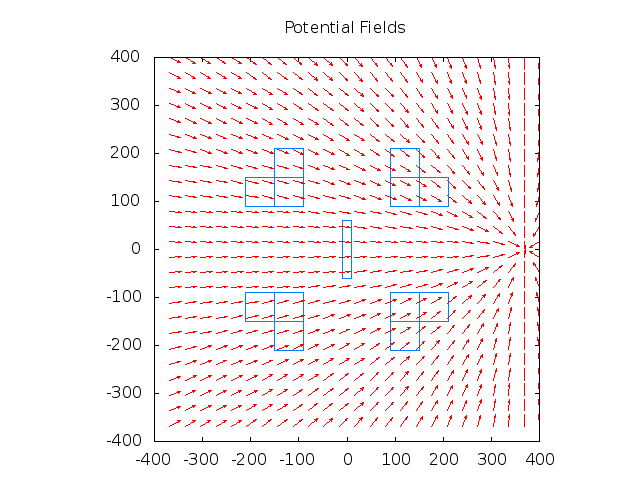
\includegraphics[width=.24\textwidth]{plots/four_ls/pfFlag.png}}
	\subfigure[Repulsive around obstacles]{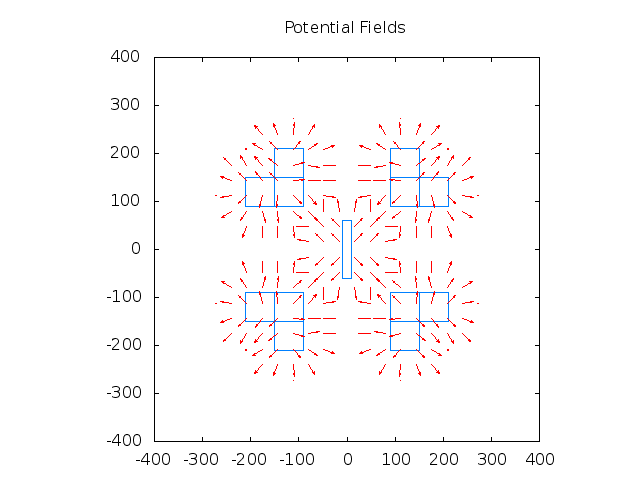
\includegraphics[width=.24\textwidth]{plots/four_ls/pfObstacles.png}}
	\subfigure[Tangential around obstacles]{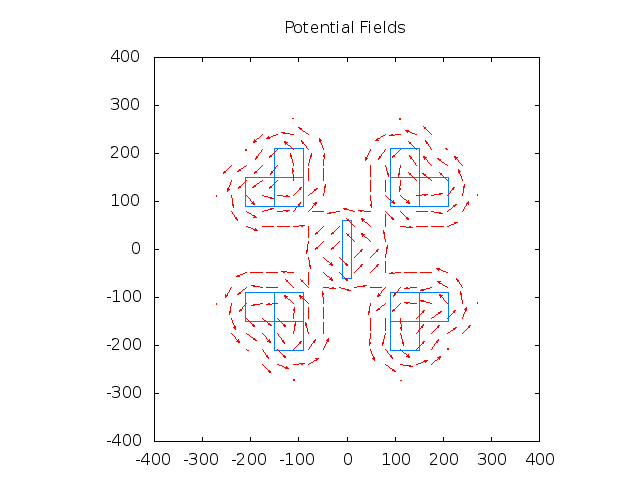
\includegraphics[width=.24\textwidth]{plots/four_ls/pfObstaclesTangential.png}}
	\subfigure[Attractive and repulsize]{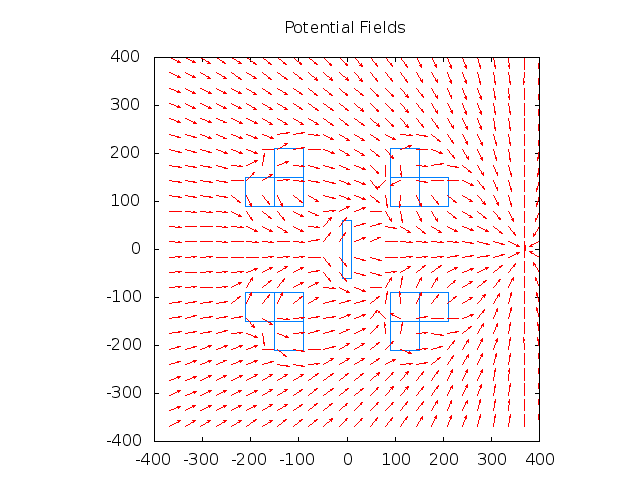
\includegraphics[width=.24\textwidth]{plots/four_ls/pfFlagsAndObstacles.png}}
	\caption{Potential fields in the FourLS World}
\end{figure}

\subsection{rotated squares}

\begin{figure}[h]
	\subfigure[Attractive Fields]{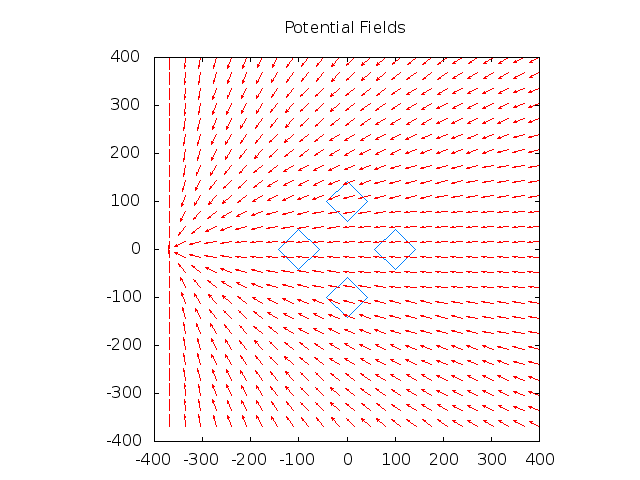
\includegraphics[width=.24\textwidth]{plots/rotated_box_world/pfFlag.png}}
	\subfigure[Repulsive Fields]{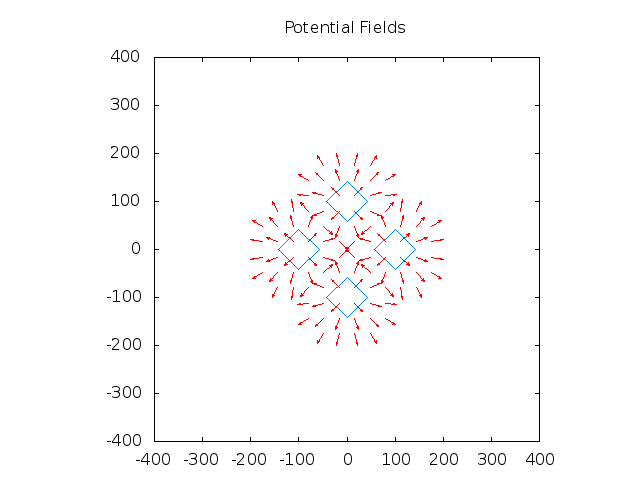
\includegraphics[width=.24\textwidth]{plots/rotated_box_world/pfObstacles.png}}
	\subfigure[Tangential Fields]{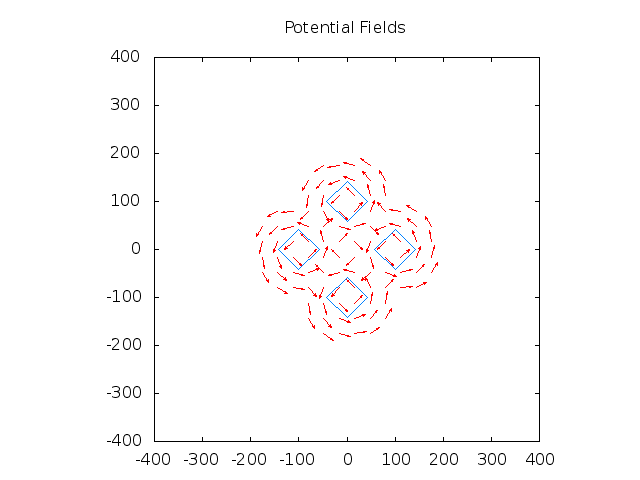
\includegraphics[width=.24\textwidth]{plots/rotated_box_world/pfObstaclesTangential.png}}
	\subfigure[Attractive and Tangential]{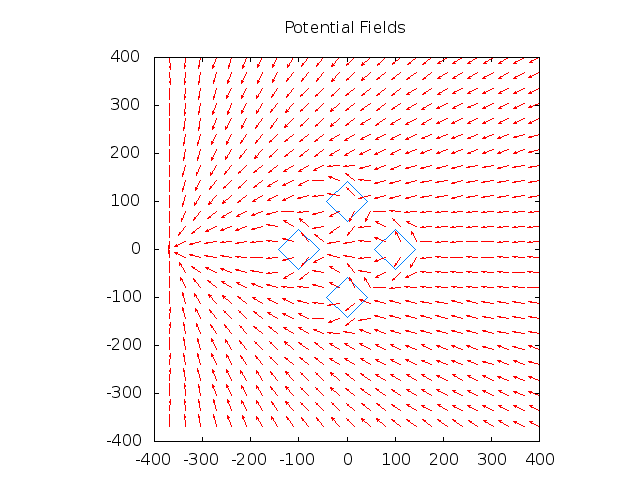
\includegraphics[width=.24\textwidth]{plots/rotated_box_world/pfFlagsAndObstacles.png}}
	\caption{Potential fields in the rotated box world}
\end{figure}

\section{Tests}
We tested our agent against Daniel Brown and Ryan Hintze's agent.
Our PF agent lost against theirs.
We had our PF agent going really slow to guarantee that he followed the field path.
After we ran the tests, we tweaked the values of the different fields as well as our controller and were significantly able to increase speed.

\section{Controller}
For turning we used a PD controller that slows the tank down to $.6$ while turning and then resets the speed to $1$ when we are going in the right direction.
We have $K_p = 1$, $K_d = 4.5$, the angle error tolerance at $2 \deg$.
As the tank gets closer to the flag, he slows down to not over shoot the flag.

\section{Time Spent}
Taylor spent about 20 hours, with about 2 hours getting used to the language (Scala).
Tyler spent about 17 hours.
\end{document}
